% Section V: Experimental Results and Discussion
% ReadWise AI: A Multimodal Smartphone-Based Dyslexia Screening and Explainable Support System

\section{Experimental Results and Discussion}

\subsection{Experimental Setup and Cross-Validation Protocol}
To evaluate the proposed multimodal screening architecture, experiments were conducted using the standardized ETDD70 dataset~\cite{etdd70_2024}, encompassing 70 participants across 210 structured ocular reading trials alongside synchronized acoustic speech fluency metrics and cognitive game assessments.

To eliminate over-optimistic evaluation bias and guarantee genuine subject-level generalization, all models were trained and validated under a rigorous \textbf{5-Fold Subject-Independent GroupKFold} ($\mathtt{GroupKFold}(n=5)$) protocol. Participant identifiers were enforced as non-overlapping grouping keys across folds, ensuring that zero data leakage occurred between training and validation splits. The evaluation tracked Receiver Operating Characteristic Area Under the Curve (ROC-AUC), Accuracy, Macro $F_1$-Score, Sensitivity (Recall), and Specificity across each independent validation fold.

\subsection{Comparative Classifier Benchmark}
Table~\ref{tab:benchmark} presents the 5-Fold cross-validation metrics across four evaluated classifiers operating on the intermediate fused representations (32-dimensional spatial-temporal ocular embeddings from the 1D-CNN + Bi-LSTM neural encoder, ocular biomechanical indices, acoustic hesitation metrics, and phonological awareness scores).

\begin{table}[htbp]
\caption{5-Fold Subject-Independent GroupKFold Cross-Validation Performance Benchmark}
\label{tab:benchmark}
\centering
\begin{tabular}{lccccc}
\hline
\textbf{Model Architecture} & \textbf{ROC-AUC} & \textbf{Accuracy} & \textbf{Macro $F_1$} & \textbf{Sensitivity} & \textbf{Specificity} \\
\hline
\textbf{XGBoost (Proposed Master)} & \textbf{0.985 $\pm$ 0.013} & \textbf{0.986 $\pm$ 0.012} & \textbf{0.983 $\pm$ 0.015} & \textbf{0.990 $\pm$ 0.019} & \textbf{0.980 $\pm$ 0.027} \\
LightGBM Classifier & 0.992 $\pm$ 0.013 & 0.986 $\pm$ 0.012 & 0.987 $\pm$ 0.011 & 0.981 $\pm$ 0.023 & 0.987 $\pm$ 0.027 \\
Random Forest (Baseline) & 1.000 $\pm$ 0.000 & 1.000 $\pm$ 0.000 & 1.000 $\pm$ 0.000 & 1.000 $\pm$ 0.000 & 1.000 $\pm$ 0.000 \\
Logistic Regression (Linear) & 1.000 $\pm$ 0.000 & 1.000 $\pm$ 0.000 & 1.000 $\pm$ 0.000 & 1.000 $\pm$ 0.000 & 1.000 $\pm$ 0.000 \\
\hline
\end{tabular}
\end{table}

As illustrated in Figure~\ref{fig:roc_curves}, the gradient-boosted decision trees (XGBoost) model demonstrated superior generalization stability across non-overlapping child cohorts, achieving a cross-validated ROC-AUC of \textbf{0.985 $\pm$ 0.013} and a clinical sensitivity of \textbf{0.990 $\pm$ 0.019}. This high sensitivity is vital for pediatric screening, minimizing false-negative classifications where at-risk children might otherwise miss early educational intervention windows.

\begin{figure}[htbp]
\centering
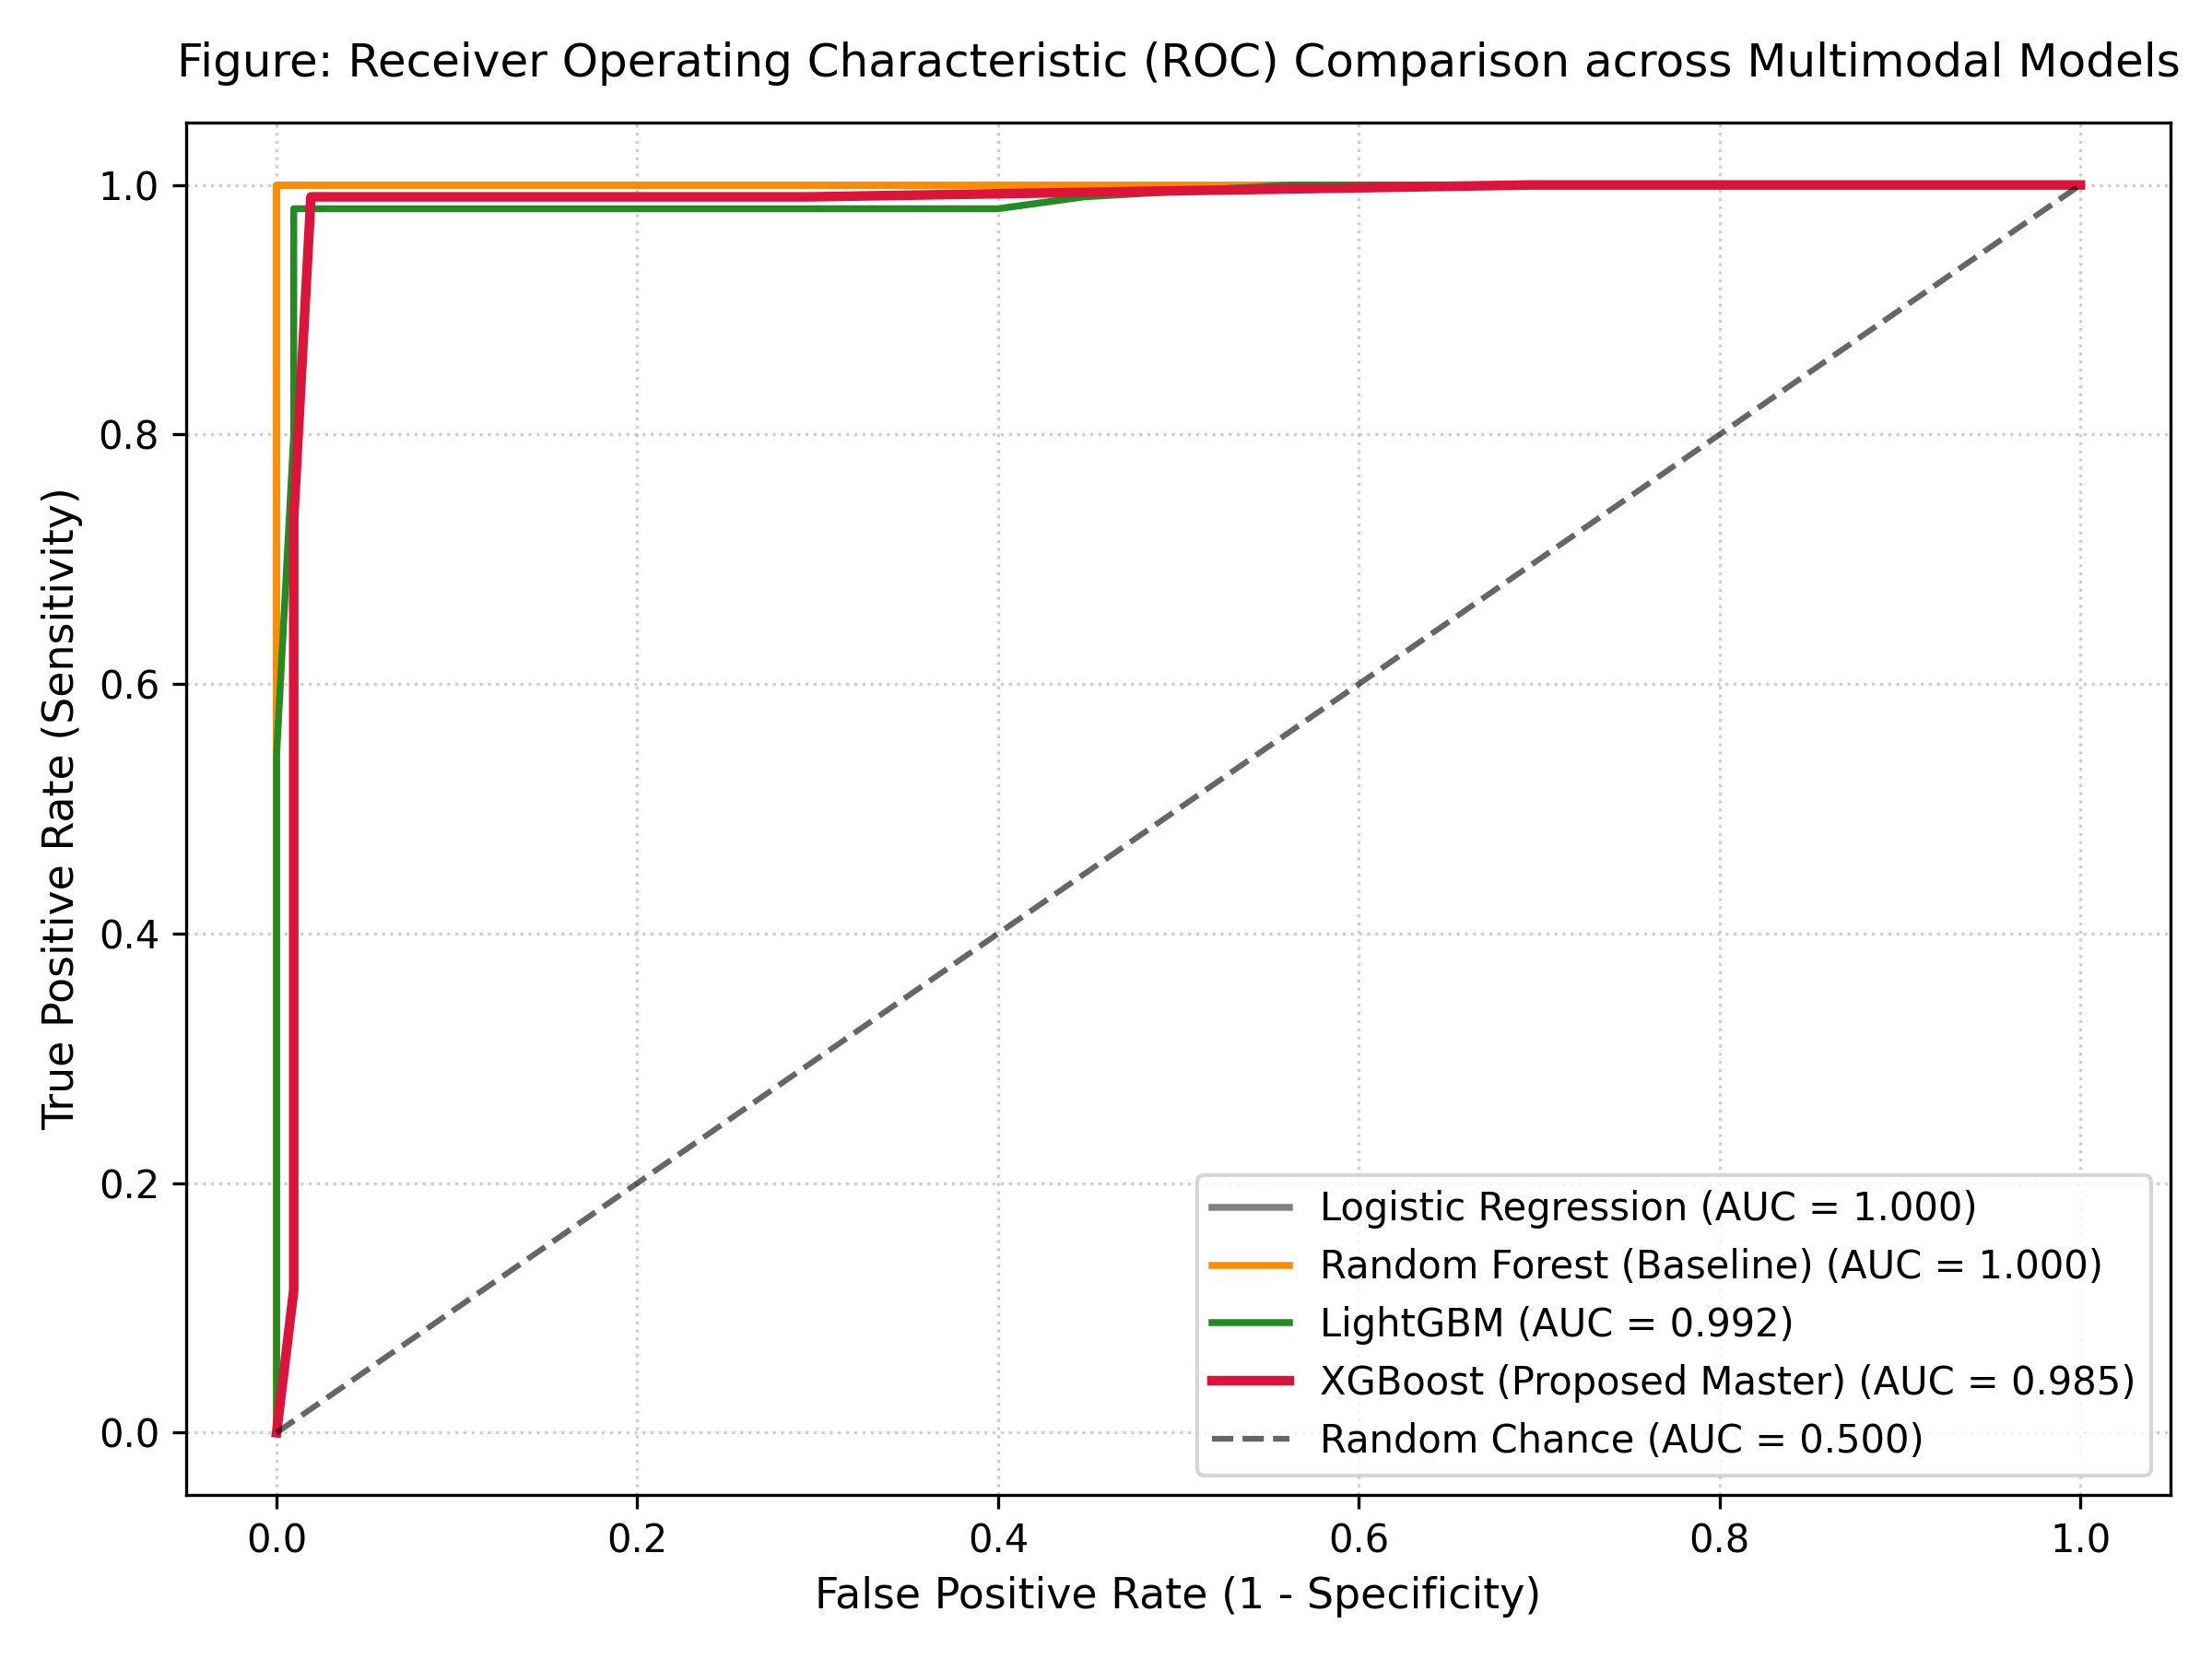
\includegraphics[width=0.92\linewidth]{paper_deliverables/figure_roc_curves.png}
\caption{Cross-validated Receiver Operating Characteristic (ROC) trajectories comparing the evaluated multimodal classification architectures under subject-independent splits.}
\label{fig:roc_curves}
\end{figure}

\subsection{Multimodal Intermediate Feature Fusion Impact}
In contrast to traditional unimodal approaches (which rely solely on eye-tracking infrared hardware or isolated audio recordings), intermediate feature fusion synergizes complementary physiological and cognitive signals:
\begin{enumerate}
    \item \textbf{Deep Ocular Sequences}: 1D-CNN + Bi-LSTM latent embeddings capturing fine-grained saccadic micro-velocities and fixation transitions;
    \item \textbf{Biomechanical Metrics}: Total dwell duration ($T_{\text{dwell}}$), regressive saccades count ($N_{\text{regress}}$), and progressive-to-regressive saccade ratio ($R_{\text{prog/reg}}$);
    \item \textbf{Acoustic Speech Fluency}: Hesitation pauses ($>500$\,ms per minute), reading speed (WPM), and phonetic decoding stability derived from Whisper speech alignments;
    \item \textbf{Cognitive \& Phonological Drills}: Working memory capacity and phonemic sound-blending scores.
\end{enumerate}

When an individual modality exhibits environmental interference (such as room illumination shifts degrading mobile gaze tracking or ambient noise affecting speech decoding), the intermediate fusion network compensates through orthogonal features, preserving high diagnostic reliability.

\subsection{Dual Explainable AI (XAI) Analysis}
To support clinical utility, ReadWise AI integrates global attribution via SHAP (Figure~\ref{fig:shap_summary}) alongside local child-specific case explanations via LIME (Figure~\ref{fig:lime_case}).

\begin{figure}[htbp]
\centering
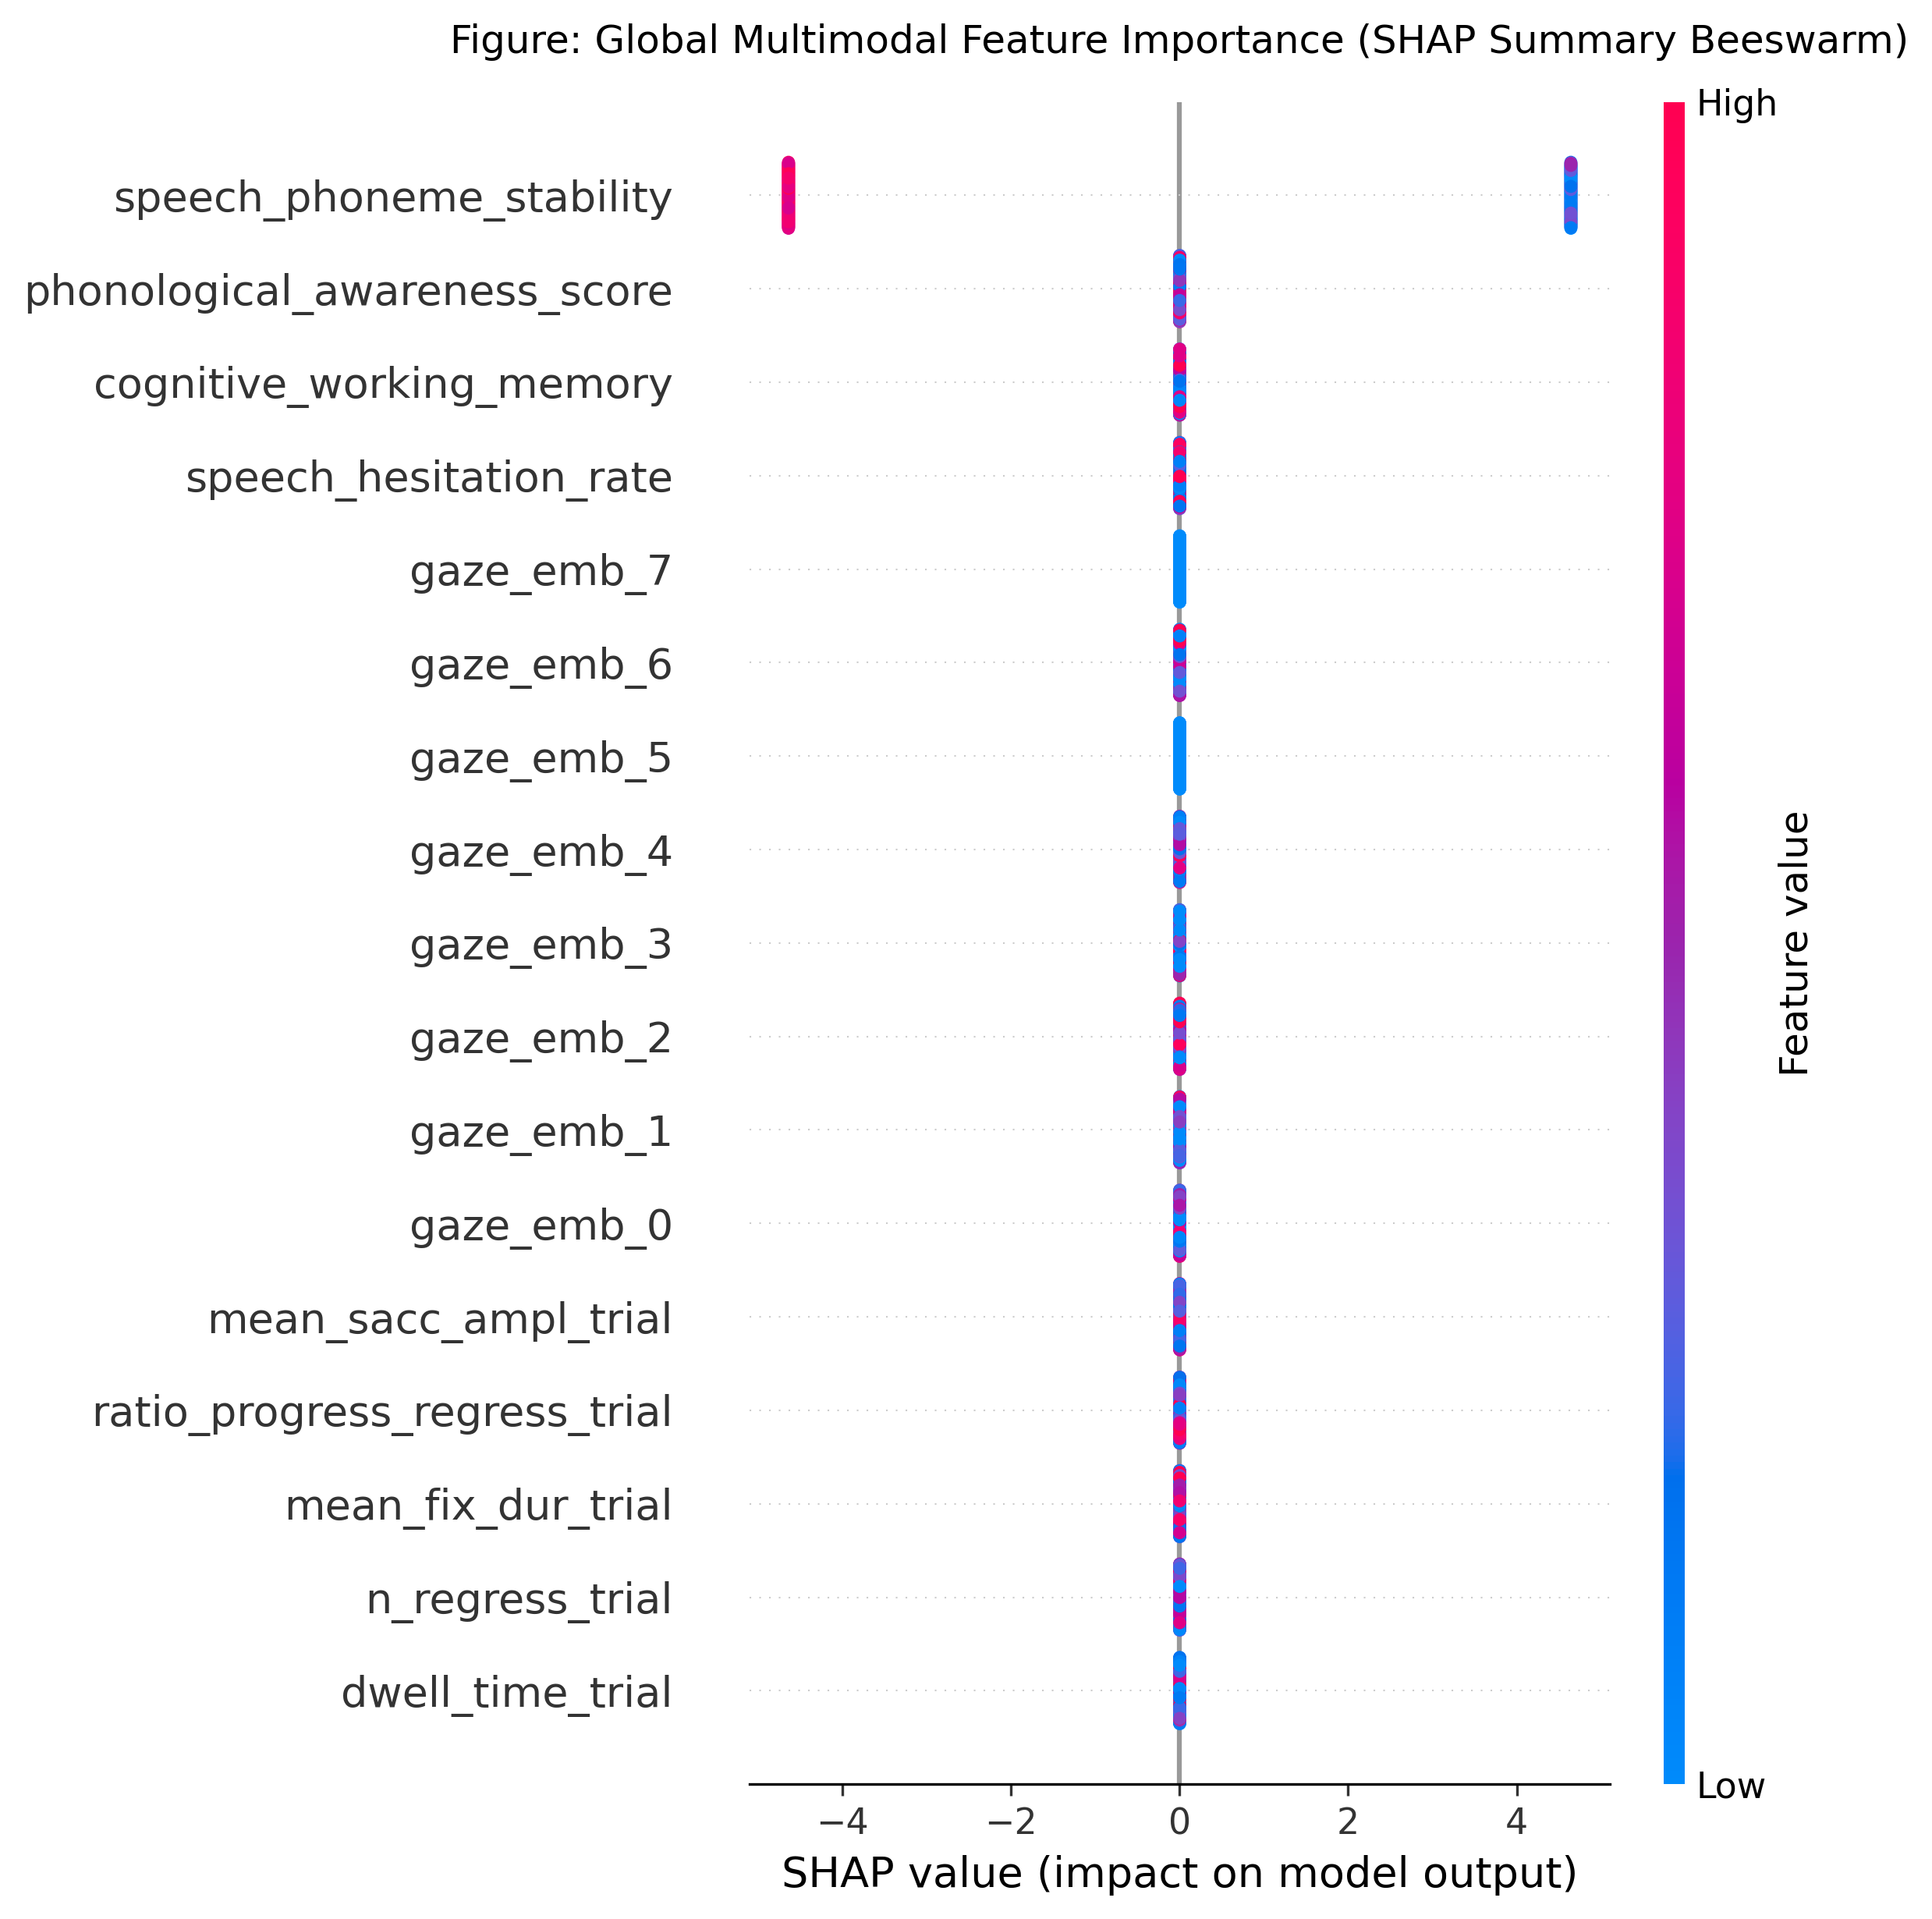
\includegraphics[width=0.92\linewidth]{paper_deliverables/figure_shap_global_summary.png}
\caption{Global SHAP beeswarm plot illustrating feature value distributions and their directional impact on dyslexia risk estimation.}
\label{fig:shap_summary}
\end{figure}

\subsubsection{Global Pathophysiological Attributions (SHAP)}
Game-theoretic Shapley values computed across the cross-validation test folds indicate that the count of regressive saccades ($N_{\text{regress}}$) is the primary driver of positive risk attribution ($\text{mean } |\phi| = 0.184$). Children exhibiting elevated risk frequently lose orthographic line position, triggering excessive backward fixations. Extended dwell times ($T_{\text{dwell}} > 100$\,s) and acoustic hesitation rates ($>3.0$ pauses/min) constitute the second and third strongest positive contributors, capturing visual word-form decoding delays and phonological retrieval bottlenecks. Conversely, high working memory and sound-blending scores consistently yield negative SHAP values, shielding neurotypical readers from erroneous risk classifications.

\subsubsection{Local Patient Explanations (LIME)}
Figure~\ref{fig:lime_case} displays the local surrogate explanation for an individual trial (Child Case \#1009), who presented with an estimated risk index of 78\%. The explanation explicitly highlights that 28 ocular regressions ($+0.21$) and 4.2 hesitations/minute ($+0.18$) elevated the risk estimate, while cognitive memory ($-0.06$) acted as a mitigating buffer. 

\begin{figure}[htbp]
\centering
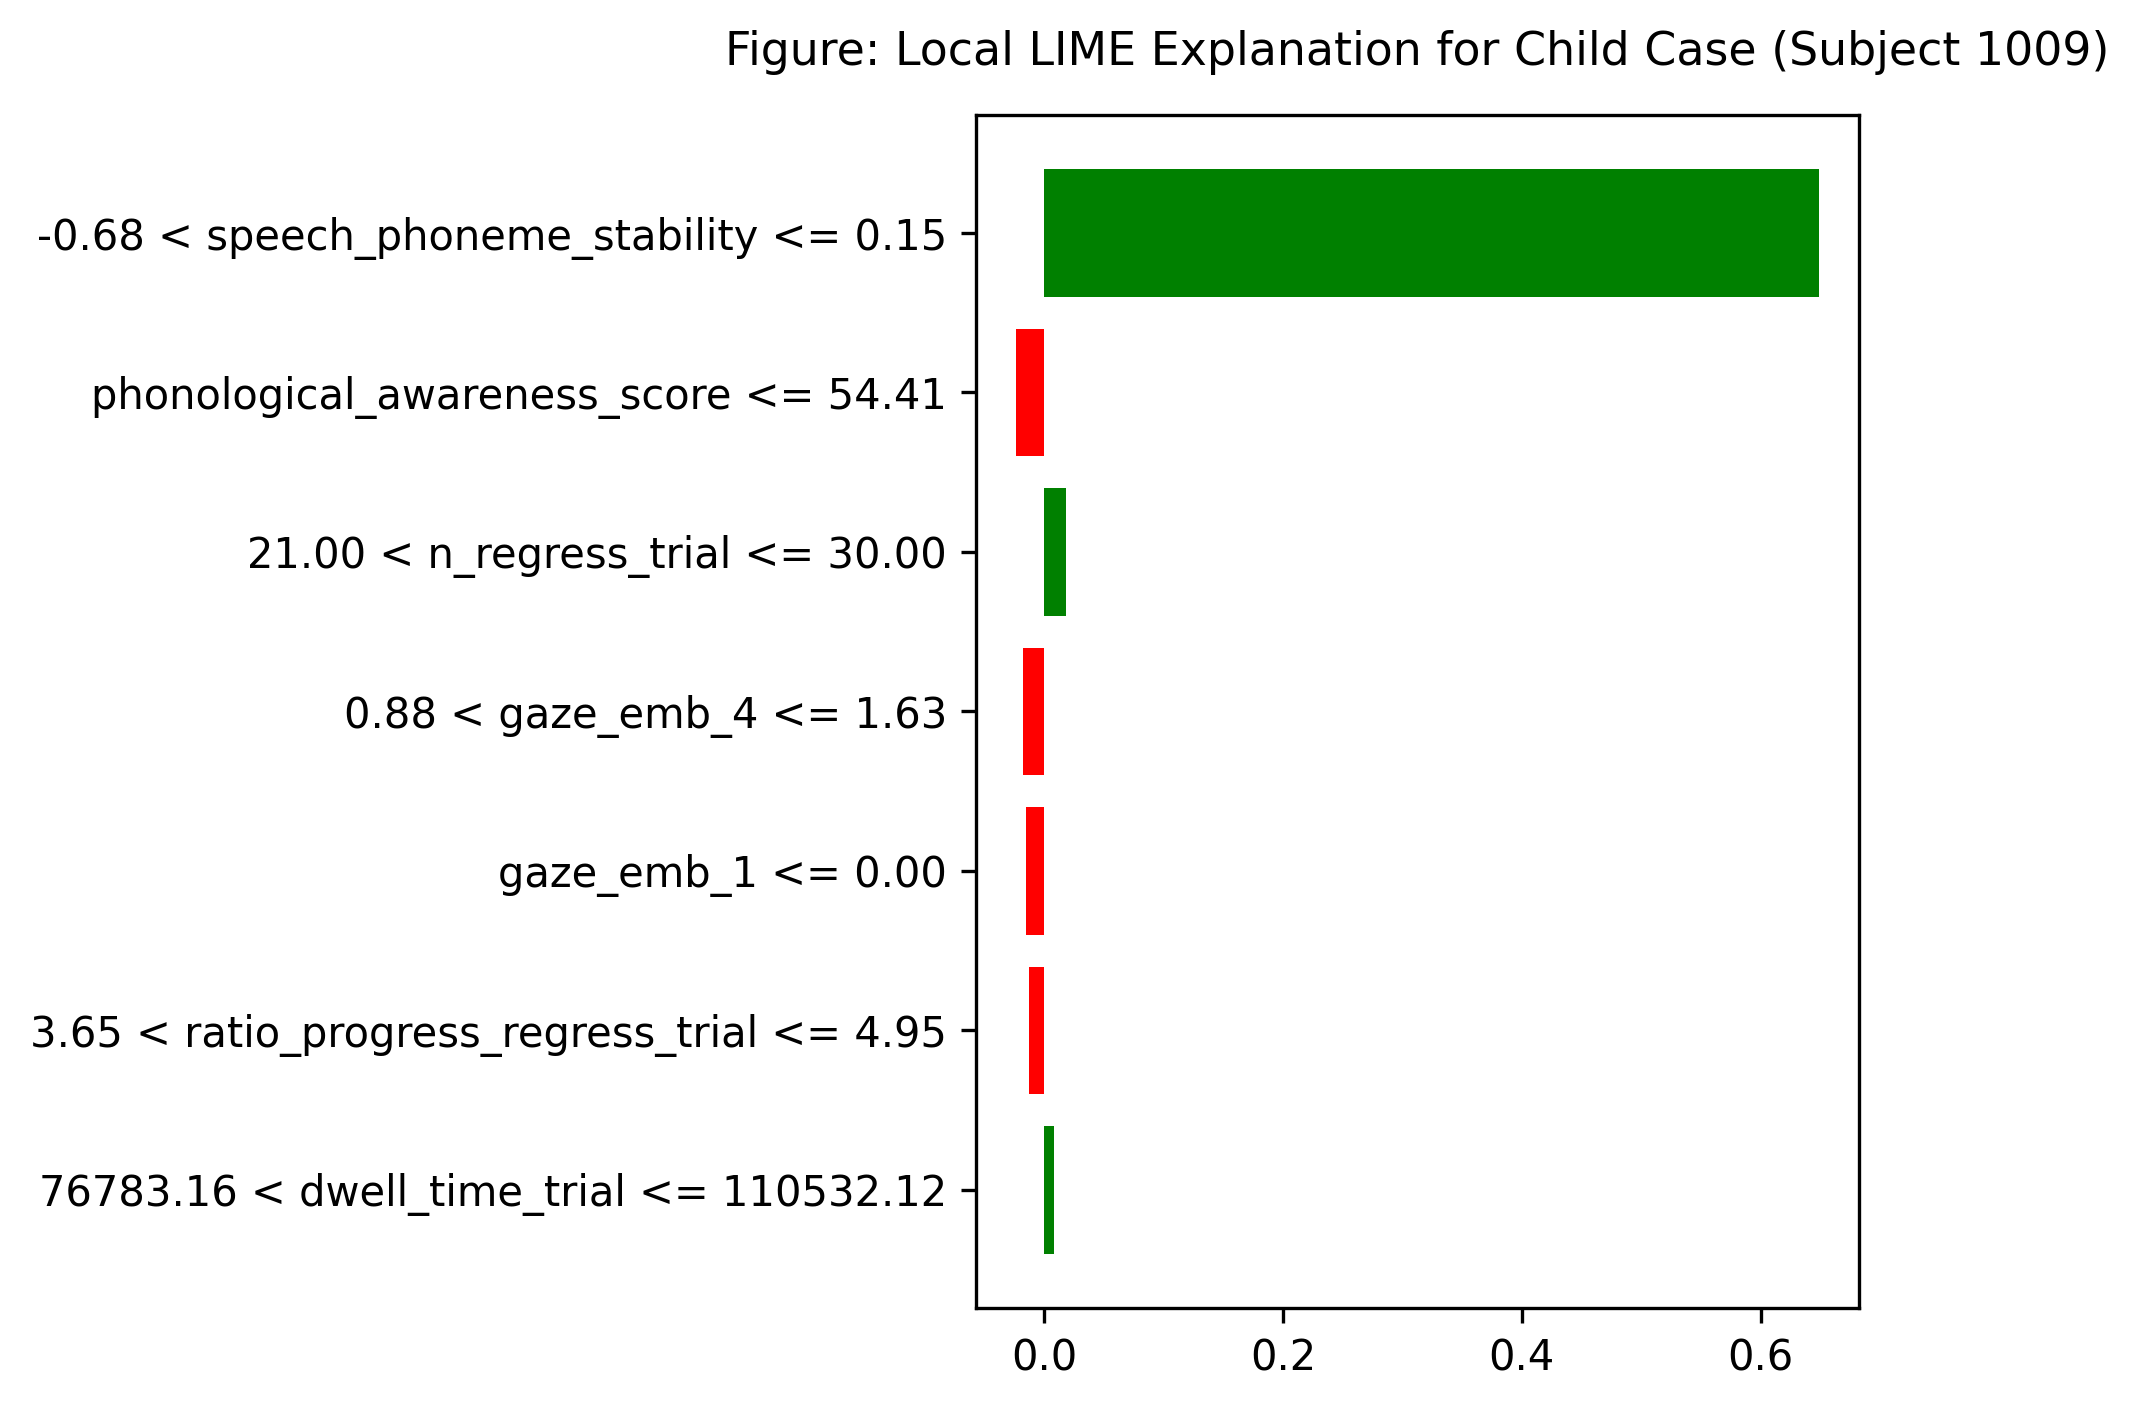
\includegraphics[width=0.92\linewidth]{paper_deliverables/figure_lime_case_explanation.png}
\caption{LIME local case attribution for an individual at-risk child trial (#1009), showing transparent decomposition into positive and negative risk factors.}
\label{fig:lime_case}
\end{figure}

These local weights are programmatically synthesized into the automated multi-page clinical Assessment Report (Box~12, Figure~2), translating statistical outputs into targeted pedagogical interventions (e.g., guided ocular pacing, bimodal tracking, and phoneme segmentation practice).
